\section{Introduction}
\label{sec:intro}

%% Maybe use some of this from SOLSTICE?
%% Today's datacenters aggregate tremendous amounts of compute and storage
%% capacity, driving demand for network switches with ever-increasing port counts
%% and line speeds.  However, supporting these demands with existing packet
%% switching technology is becoming increasingly expensive---in cost, heat, power,
%% and cabling. Packet switches are flexible, capable of making forwarding
%% decisions at the granularity of individual packets.  In common modern scenarios,
%% however, this flexibility is unnecessary: many (often consecutive) packets are
%% sent to the same output port.  Two key factors contribute to this traffic
%% pattern. First, traffic inside a datacenter often has high spatial locality,
%% where a large fraction of the traffic that enters each switch port is destined
%% for only a small number of output ports~\cite{msft-imc09, facebook:sigcomm15}.
%% Second, traffic is often bursty, with significant temporal locality between
%% packets sharing the same destination~\cite{bullet:conext13,
%%   facebook:sigcomm15}. The consequence of these two factors is that the traffic
%% demand matrix at a datacenter switch is often both skewed and
%% sparse~\cite{mordia:hotnets12,flyways,augmenting-dc-wireless}.

%% \begin{figure*}[t!!!]
%% \centering
%% 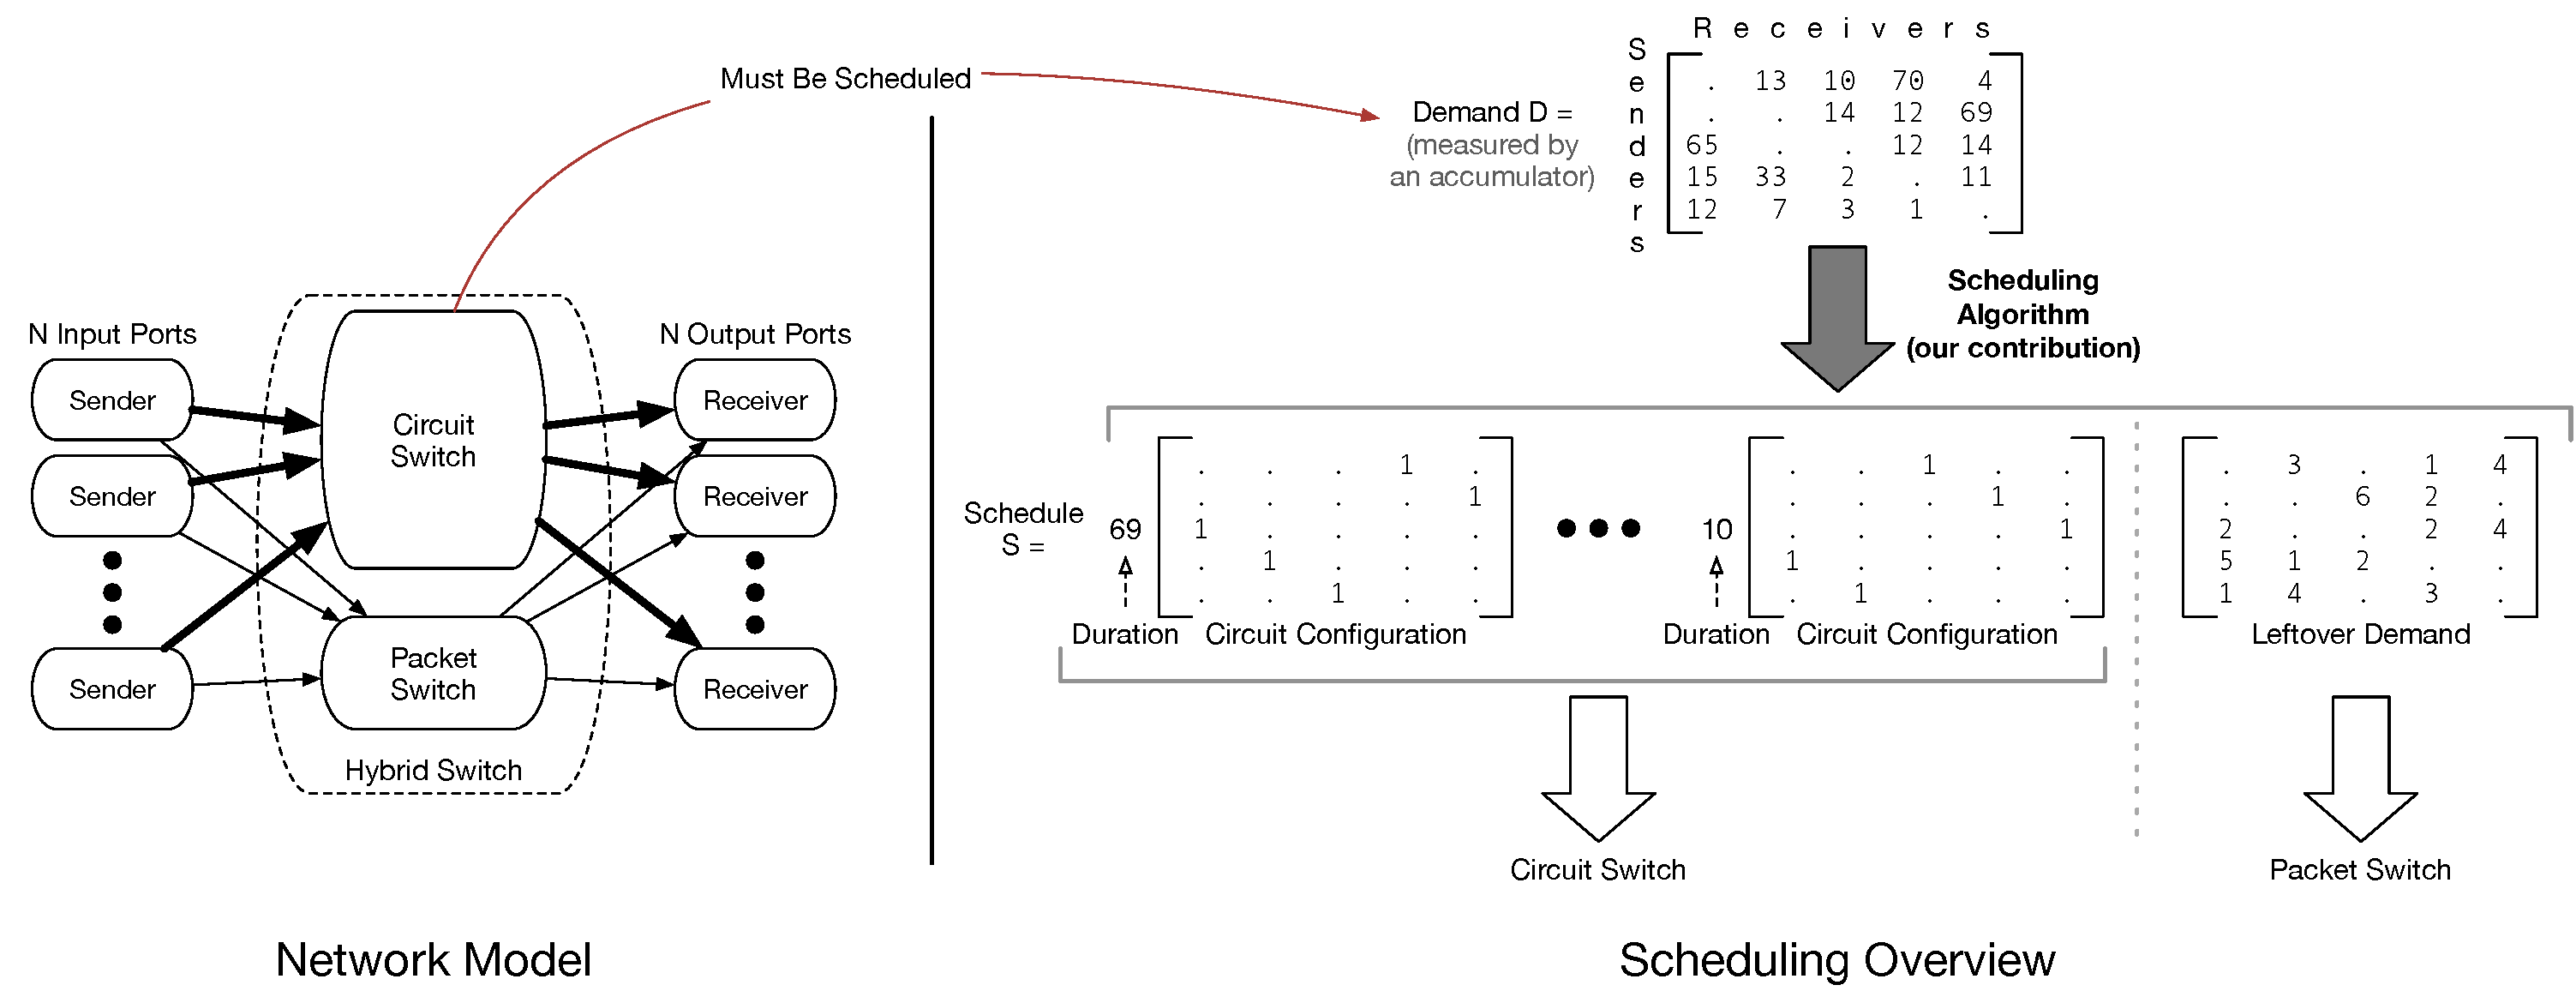
\includegraphics[width=1\textwidth]{figures/setting}
%% \caption{Our model of a hybrid switch architecture and the scheduling
%%   process. The circuit switch has high bandwidth, but slow reconfiguration
%%   time. The packet switch has low bandwidth (e.g., an order of magnitude lower),
%%   but can make forwarding decisions per-packet.
%%   %Both switches must have high utilization.
%%   }
%% \label{fig:arch}
%% \end{figure*}

%% Researchers have seized upon these observations to propose hybrid datacenter
%% network architectures that offer higher throughput at lower cost by combining
%% high-speed optical~\cite{OSA,helios:sigcomm10,c-Through} or
%% wireless~\cite{flyways,augmenting-dc-wireless,mirror-mirror} circuit switching
%% technologies with traditional electronic packet switches. Typically, the circuit
%% switch has a significantly higher data rate than the packet switch, but incurs a
%% non-trivial reconfiguration penalty. While the potential cost savings that
%% hybrid techniques could realize is large, the design space of scheduling
%% algorithms that enable high utilization in hybrid networks is not yet well
%% understood. Earlier work that considers circuit switches with substantial
%% reconfiguration delay offers no guidance about how to negotiate the trade-off
%% between remaining in the current (potentially sub-optimal) circuit configuration
%% vs. incurring a costly reconfiguration delay to switch to a potentially better
%% circuit configuration~\cite{c-Through, helios:sigcomm10, wang:hotnets}.  The
%% reconfiguration cost of these systems was so high that they were forced to keep
%% a configuration pinned up for a relatively long period anyway.

%% In recent years, however, the switching time of optical circuit switches has
%% improved substantially~\cite{mordia:sigcomm13}. As a result, an efficient
%% scheduling algorithm for a modern hybrid design must determine: 1) a set of
%% circuit configurations (which ports are connected to which other ports and how
%% long that configuration should remain in effect) designed to maximize the
%% traffic serviced over the high-bandwidth but slow-to-reconfigure
%% circuit-switched network, and 2) what traffic should be sent to the
%% low-bandwidth but flexible packet switch.

%% Computing an optimal set of circuit configurations to maximize circuit-switched
%% utilization has no known polynomial-time algorithms, scaling as $O(n!)$ in the
%% number of switch ports (\S\ref{sec:optimization}). The challenge arises due to
%% the non-trivial switching time between configurations, which necessitates not
%% only sending as much traffic as possible, but doing so in the fewest number of
%% configurations.

%% The end goal of this paper is an effective and fast heuristic algorithm that
%% delivers high switch utilization. To this end, we first provide a detailed
%% characterization of the problem plus an optimal (but impractical) solution that
%% sheds light on how to design an effective heuristic.  We then present our
%% heuristic, Solstice, which provides 2.9$\times$ higher utilization compared to
%% previous algorithms by taking advantage of the known sparsity and skew of
%% datacenter workloads---some of the same features that make the traditional
%% scheduling problem hard.

%% The contributions of this work are as follows:
%% \begin{enumerate}
%% \item Characterizing the hybrid switch scheduling problem.
%% \item Exploring the design space of hybrid scheduling:
%%   \begin{packedenumerate}
%%     \item \myparatight{Lower bound} an instantly computable but loose bound on
%%       the minimum amount of time it takes to serve all demand (but provides no
%%       actual schedules).
%%     \item \myparatight{Optimal scheduling} optimally schedule all
%%       demand with minimal time; impossible to run in real time at scale.
%%     \item \myparatight{Heuristic algorithm (``Solstice'')} runs in real time at
%%       scale, but slightly underperforms optimal (by at most 14\%
%%       at target scale).
%%     \item \myparatight{Heuristic + optimization (``\mbox{Solstice{}++}'')} runs at
%%       scale (though not in real time), but tightens the gap between Solstice and
%%       optimal (at most 12\% from optimal at target scale).
%%   \end{packedenumerate}
%% \item Insight into the challenges and benefits of using hybrid switches, with a
%%   focus on high circuit utilization.
%% \end{enumerate}
